\documentclass[border=6pt]{standalone}
\usepackage[T1]{fontenc}
\usepackage{courier}
\usepackage[scaled=0.95]{helvet}
\renewcommand{\familydefault}{\sfdefault}
\usepackage{sfmath}
\usepackage[version=4]{mhchem}
\usepackage{tikz}
\usepackage{pgfplots}
\pgfplotsset{compat=newest}
\usetikzlibrary{arrows.meta,positioning,calc,fit,backgrounds,shapes.geometric,decorations.pathreplacing,patterns}
\definecolor{ink}{HTML}{17233A}
\definecolor{inksoft}{HTML}{44506A}
\definecolor{teal}{HTML}{0E6B6B}
\definecolor{tealsoft}{HTML}{E5F0EF}
\definecolor{amber}{HTML}{B26B12}
\definecolor{ambersoft}{HTML}{FBF0DF}
\definecolor{blue}{HTML}{2F6690}
\definecolor{bluesoft}{HTML}{E3ECF4}
\definecolor{plum}{HTML}{7A4D8C}
\definecolor{plumsoft}{HTML}{EFE7F3}
\definecolor{greyc}{HTML}{8A94A3}
\definecolor{linec}{HTML}{D3DCE1}
\definecolor{oxy}{HTML}{C0392B}
\definecolor{carb}{HTML}{3B4252}
\definecolor{hyd}{HTML}{E6E9EE}
\definecolor{nit}{HTML}{2F6690}
\tikzset{
  every picture/.style={line cap=round,line join=round},
  lab/.style={font=\small, text=inksoft},
  >={Stealth[length=7pt]},
}
\pgfplotsset{
  every axis/.append style={axis line style={inksoft}, tick style={inksoft}, tick label style={font=\footnotesize, text=inksoft}, label style={font=\small, text=ink}},
}
% fragment tile: \frag{node name}{position}{colour}{content}
\newcommand{\frag}[4]{\node[draw=#3, fill=#3!12, line width=1.4pt, rounded corners=6pt, minimum width=1.25cm, minimum height=1.05cm, text=#3, font=\bfseries] (#1) at (#2) {#4};}
\newcommand{\ring}{\tikz[baseline=-0.6ex]{\draw[line width=1.1pt] (0:0.3)--(60:0.3)--(120:0.3)--(180:0.3)--(240:0.3)--(300:0.3)--cycle; \draw[line width=0.8pt] (0,0) circle (0.16);}}
\newcommand{\bond}[2]{\draw[ink, line width=2.2pt] (#1) -- (#2);}

\begin{document}
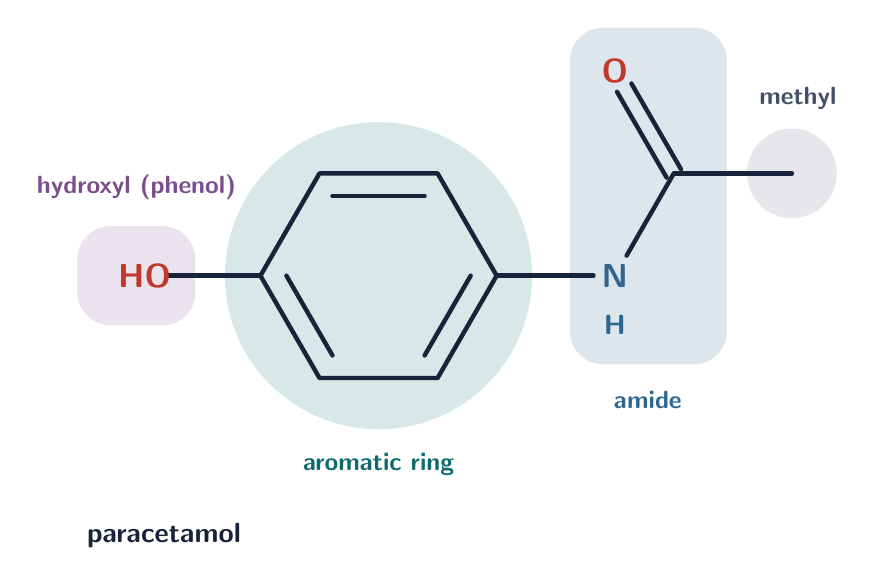
\begin{tikzpicture}[scale=1.5]
\fill[plum, fill opacity=0.16, rounded corners=12pt] (-2.55,-0.42) rectangle (-1.55,0.42);
\fill[teal, fill opacity=0.16] (0,0) circle (1.3);
\fill[blue, fill opacity=0.16, rounded corners=12pt] (1.62,-0.75) rectangle (2.95,2.1);
\fill[greyc, fill opacity=0.22] (3.5,0.866) circle (0.38);
\draw[ink, line width=1.6pt] (1.000,0.000)--(0.500,0.866)--(-0.500,0.866)--(-1.000,0.000)--(-0.500,-0.866)--(0.500,-0.866)--cycle;
\draw[ink, line width=1.6pt] (0.390,0.675) -- (-0.390,0.675);
\draw[ink, line width=1.6pt] (-0.780,0.000) -- (-0.390,-0.675);
\draw[ink, line width=1.6pt] (0.390,-0.675) -- (0.780,0.000);
\draw[ink, line width=1.6pt] (1.000,0.000) -- (1.820,0.000);\draw[ink, line width=1.6pt] (2.100,0.170) -- (2.500,0.866);\draw[ink, line width=1.6pt] (2.500,0.866) -- (3.500,0.866);\draw[ink, line width=1.6pt] (2.439,0.831) -- (2.019,1.557);\draw[ink, line width=1.6pt] (2.561,0.901) -- (2.141,1.627);\draw[ink, line width=1.6pt] (-1.000,0.000) -- (-1.780,0.000);
\node[font=\large\bfseries, text=nit, inner sep=1pt] at (2.000,0.000) {N};
\node[font=\bfseries, text=nit] at (2.000,-0.420) {H};
\node[font=\large\bfseries, text=oxy, inner sep=1pt] at (2.000,1.732) {O};
\node[font=\large\bfseries, text=oxy, inner sep=1pt, anchor=east] at (-1.730,0.000) {HO};
\node[font=\small\bfseries, text=plum] at (-2.05,0.75) {hydroxyl (phenol)};
\node[font=\small\bfseries, text=teal] at (0,-1.6) {aromatic ring};
\node[font=\small\bfseries, text=blue] at (2.28,-1.05) {amide};
\node[font=\small\bfseries, text=inksoft] at (3.55,1.5) {methyl};
\node[font=\normalsize\bfseries, text=ink, anchor=west] at (-2.55,-2.2) {paracetamol};
\end{tikzpicture}
\end{document}
